\chapter{Recurrent Neural Networks}

Le \textbf{Recurrent Neural Networks} (RNN) costituiscono una classe di architetture neurali progettate specificamente per l’elaborazione di dati sequenziali, come segnali temporali, testi o serie temporali. A differenza delle reti neurali \textit{feed-forward}, che elaborano gli input in maniera indipendente, le RNN sono dotate di una memoria interna che evolve dinamicamente nel tempo. Questa memoria consente al modello di conservare informazioni riguardanti gli stati precedenti della sequenza, rendendo possibile la modellazione delle dipendenze temporali o contestuali tra gli elementi della serie. Tale proprietà è fondamentale in applicazioni dove il significato di un dato dipende fortemente dal contesto, come nella traduzione automatica, nel riconoscimento vocale o nella generazione di testo. L'introduzione dello stato ricorrente permette dunque di superare i limiti delle architetture tradizionali, che trattavano ogni istante temporale come isolato, senza tenere conto delle relazioni tra eventi consecutivi.

\section{Predizione sequenziale}

Consideriamo il caso di un'immagine che mostra una sfera in una determinata posizione. Una domanda naturale che potremmo porci è: \textit{quale sarà il prossimo movimento della sfera? In quale direzione si sposterà?} L'obiettivo, dunque, è predire il movimento futuro della sfera basandosi su una sequenza di osservazioni precedenti. Questo tipo di compito si adatta perfettamente all'architettura delle \textbf{Recurrent Neural Networks} (RNN), in quanto tali modelli sono in grado di mantenere uno stato interno che evolve nel tempo e che cattura le dipendenze temporali tra gli input. Nello specifico, la sfera e il suo movimento possono essere rappresentati come una sequenza temporale, dove lo stato corrente è influenzato dagli stati precedenti. Un altro esempio emblematico è il testo: possiamo infatti interpretare una frase come una sequenza di parole, dove ciascuna parola dipende in misura più o meno forte da quelle che la precedono. In tale contesto, le RNN risultano particolarmente efficaci, poiché riescono a conservare informazioni contestuali pregresse utili sia alla comprensione che alla generazione del linguaggio.

\section{Predizione della parola successiva}

Consideriamo ora la frase: \textit{This morning I took my cat for a walk}. L'obiettivo è prevedere l'ultima parola conoscendo le precedenti. Questo problema è tipico nei modelli linguistici, dove si cerca di stimare la distribuzione di probabilità condizionata per una parola data una sequenza di parole precedenti. Le RNN si rivelano utili in questo contesto, poiché riescono ad utilizzare l'intero contesto passato per calcolare la probabilità della parola successiva. Tuttavia, anche queste reti incontrano difficoltà nel trattare contesti molto lunghi, a causa di problemi noti come la \textbf{scomparsa del gradiente}, che ostacolano l’apprendimento di dipendenze a lungo termine.

\subsection{Finestra fissa}

Una strategia alternativa consiste nell'utilizzare una \textbf{finestra temporale fissa} di parole per predire la successiva. In questo caso, solo un numero limitato di parole precedenti viene considerato come input per la previsione. Tuttavia, questa scelta comporta una perdita di contesto: se la finestra è troppo piccola, il modello rischia di ignorare informazioni fondamentali; se è troppo grande, può diventare inefficiente e soggetta a instabilità, a causa del già citato problema della scomparsa del gradiente. Nel nostro esempio, se considerassimo soltanto le due parole precedenti, sarebbe molto improbabile riuscire a predire correttamente la parola finale. L’ampliamento della finestra può sembrare una soluzione, ma deve essere bilanciato per evitare un aumento eccessivo della complessità computazionale.

\subsection{One-hot encoding}

Una rappresentazione comune delle parole è il \textbf{one-hot encoding}, dove ogni parola è codificata come un vettore binario in cui un solo elemento è attivo (cioè pari a 1), mentre tutti gli altri sono a zero. Sebbene semplice, questa rappresentazione è poco efficiente dal punto di vista semantico, poiché non cattura alcuna relazione tra parole simili. Per superare tali limitazioni si introducono i \textbf{word embeddings}, rappresentazioni dense e continue che posizionano le parole in uno spazio vettoriale tale che termini semanticamente simili risultino geometricamente vicini.

\subsection{Bag of Words}

Un ulteriore approccio è il \textbf{Bag of Words} (BoW), in cui l'intera frase viene rappresentata come un vettore che indica la presenza o assenza di ogni parola, indipendentemente dalla loro posizione. Tuttavia, tale metodo ignora completamente l’ordine delle parole, il quale è invece cruciale per la comprensione sintattica e semantica del linguaggio. Un cambiamento minimo nell’ordine delle parole può alterare radicalmente il significato di una frase. Le RNN, al contrario, preservano l’ordine sequenziale degli input e permettono di modellare strutture linguistiche complesse, grazie alla loro capacità di mantenere la memoria temporale e adattarsi a dipendenze di lungo periodo.

\begin{table}[htbp]
\centering
\footnotesize
\caption{Confronto tra approcci per la rappresentazione del testo e la predizione sequenziale.}
\begin{adjustbox}{width=\textwidth}
\begin{tabular}{l|p{3.8cm}|p{3.5cm}|p{3.5cm}}
\hline
\textbf{Metodo} & \textbf{Caratteristiche principali} & \textbf{Vantaggi} & \textbf{Svantaggi} \\
\hline
\textbf{Finestra fissa} & Considera solo $n$ parole precedenti & Computazionalmente semplice & Non gestisce dipendenze a lungo termine \\
\hline
\textbf{One-hot encoding} & Rappresentazione binaria con un solo 1 attivo & Facile da implementare & Non cattura relazioni semantiche \\
\hline
\textbf{Bag of Words (BoW)} & Rappresenta la presenza o frequenza delle parole ignorando l’ordine & Semplice e interpretabile & Perde completamente l’informazione sull’ordine \\
\hline
\textbf{Word Embeddings} & Vettori densi che catturano somiglianze semantiche & Efficienza e rappresentazione semantica & Richiede training e risorse computazionali \\
\hline
\end{tabular}
\end{adjustbox}
\label{tab:metodi_sequenziali}
\end{table}

\section{Architettura delle RNN}

Le reti neurali \textit{feedforward} elaborano gli input in un'unica direzione, dall'input all'output, senza tenere conto della sequenzialità o della dipendenza temporale dei dati. In tal modo, presuppongono che ogni input e output sia indipendente dagli altri. Questa assunzione le rende inadatte a compiti in cui il contesto o l'ordine temporale sono fondamentali (es. traduzione, modellazione linguistica, riconoscimento vocale). Le Reti Neurali Ricorrenti (RNN), invece, sono progettate per lavorare su sequenze, riconoscendo pattern temporali grazie alla capacità di mantenere una \textit{memoria} implicita dello stato precedente della rete. In altre parole, una RNN può sfruttare informazioni precedenti per influenzare le previsioni successive, rendendola adatta a compiti dove la storia è rilevante.
\begin{figure}
\centering
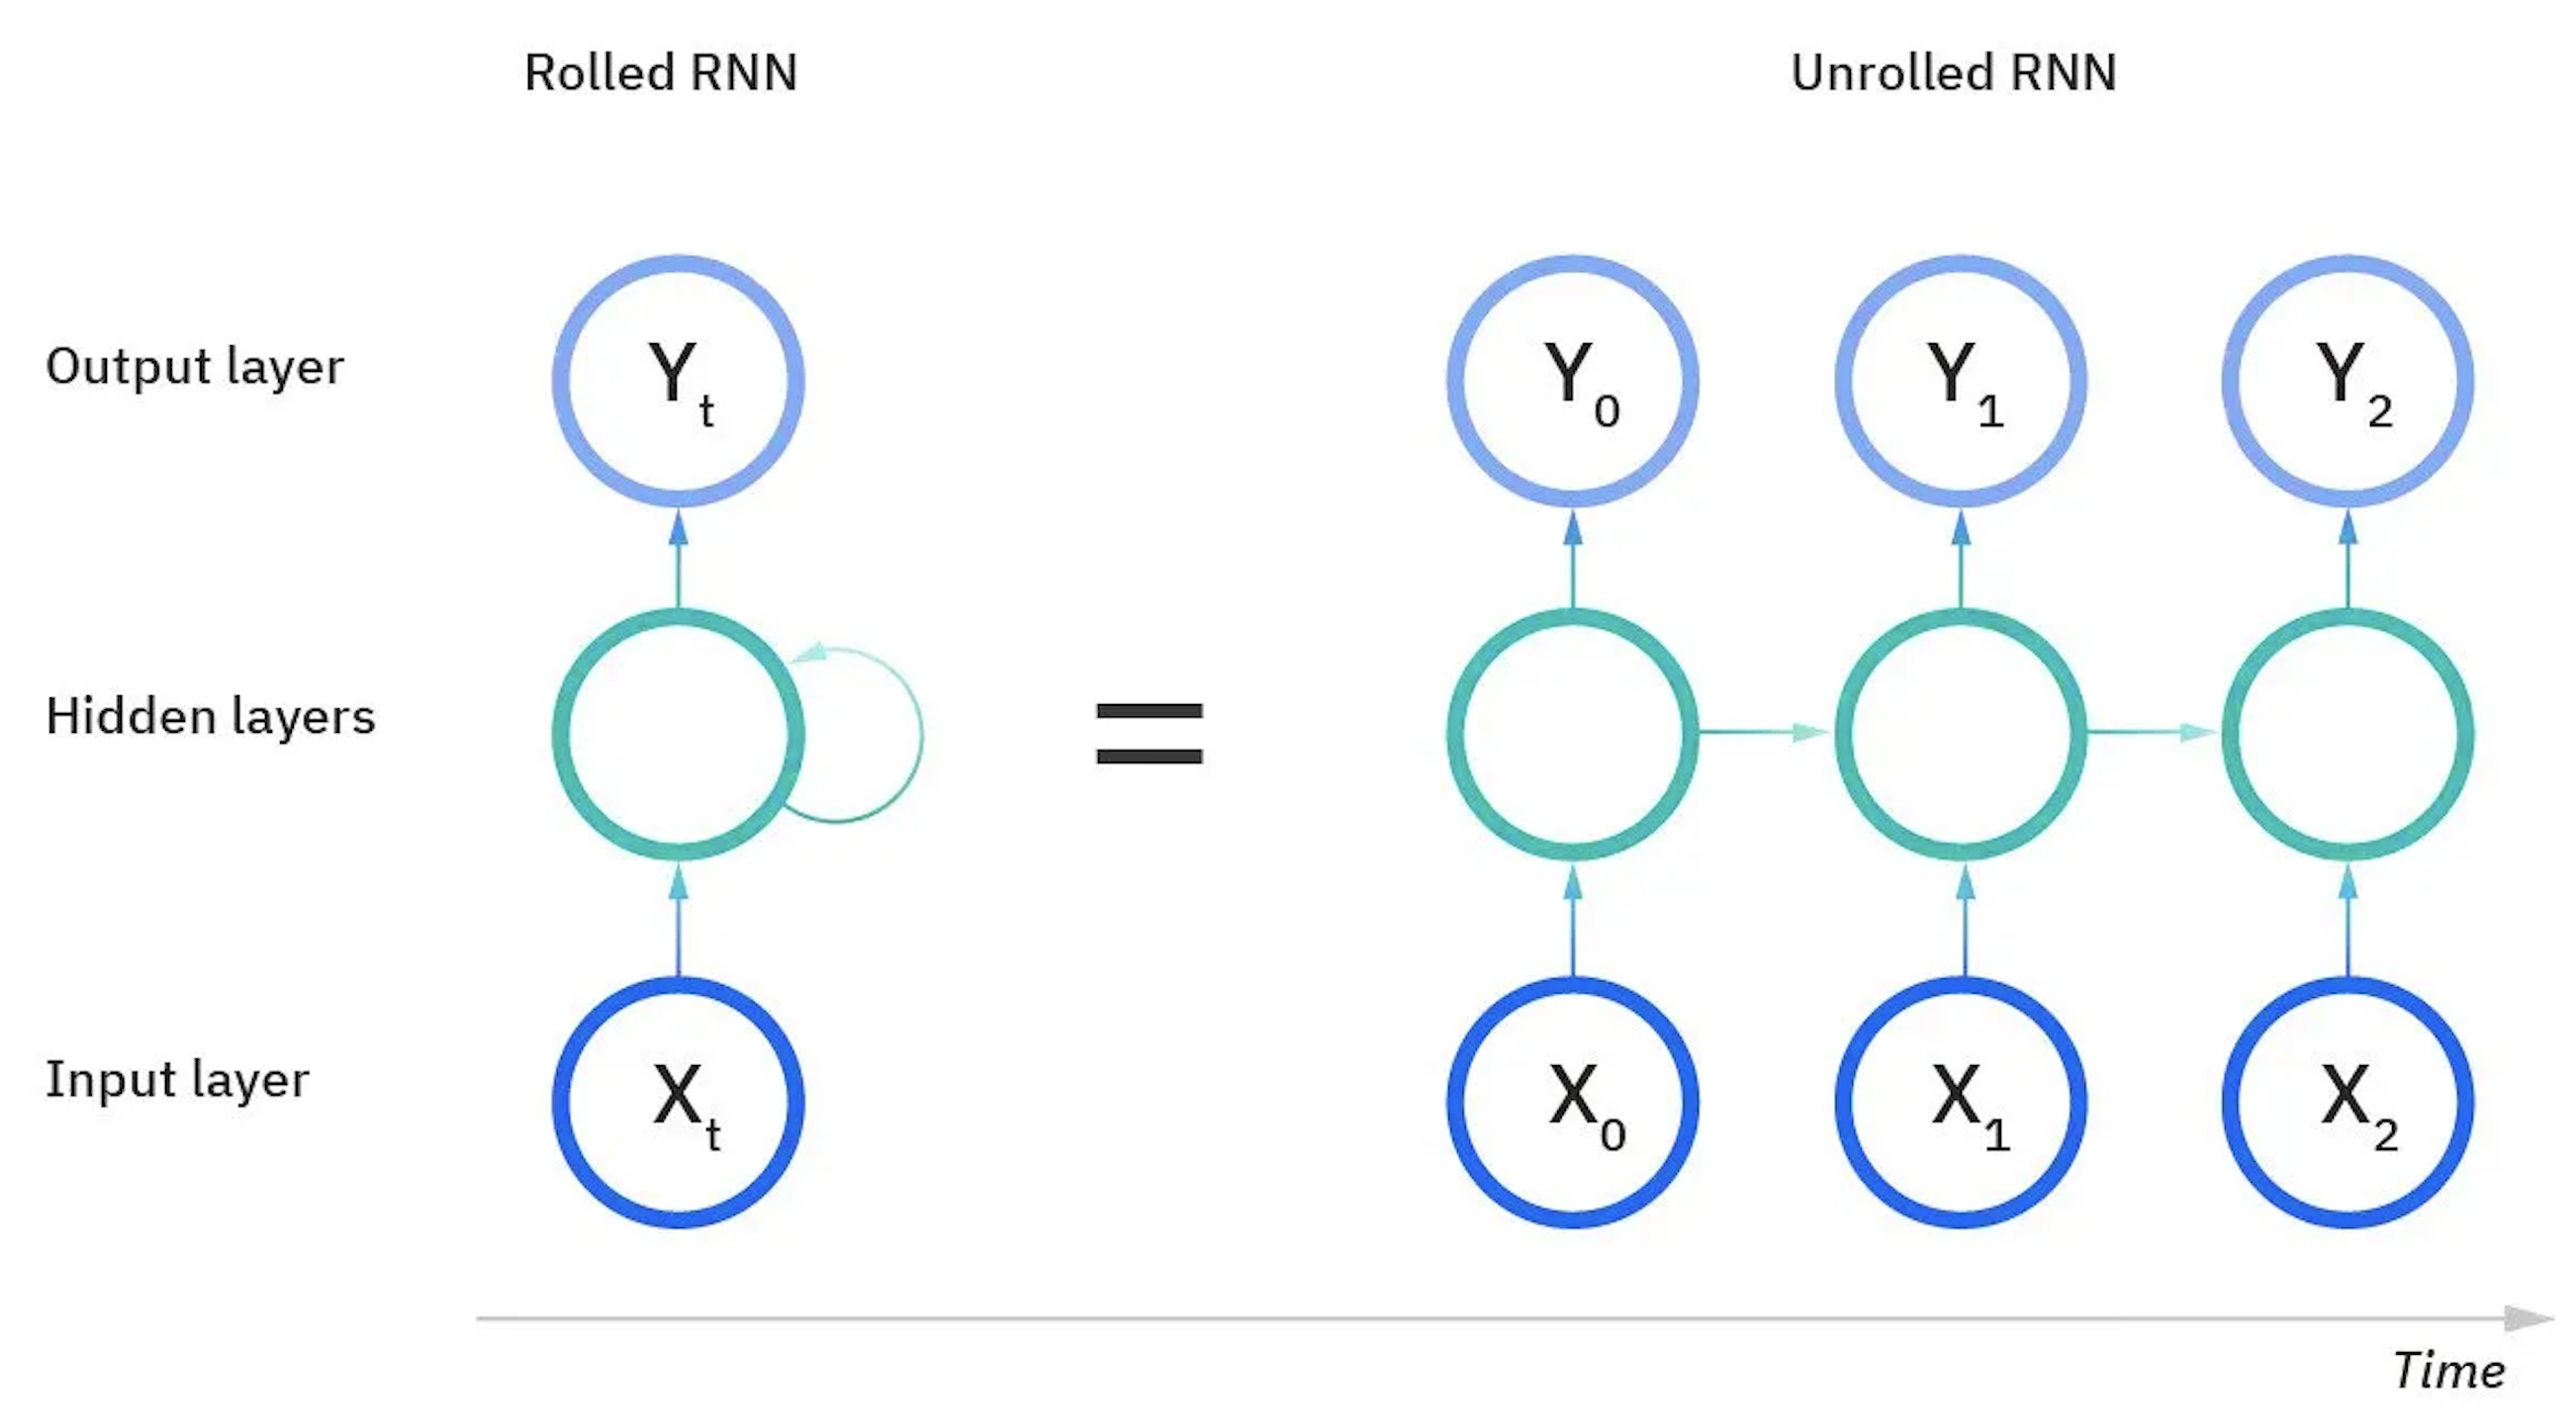
\includegraphics[width=0.70\textwidth]{figure/RNNRoll.png}
\caption{Rappresentazione schematica di una Recurrent Neural Network, nella versione "arrotolata" (a sinistra) e "srotolata" (a destra).}
\label{fig:rolledRNN}
\end{figure}
Per comprendere meglio il concetto, consideriamo l'espressione idiomatica inglese "feeling under the weather", comunemente usata per indicare che qualcuno è malato. L'espressione ha senso solo se le parole vengono pronunciate in quell'ordine specifico. Una RNN è in grado di interpretarla correttamente perché, elaborando ogni parola nel contesto delle precedenti, riesce a mantenere il significato dell'intera sequenza. La vista "arrotolata" della Figura~\ref{fig:rolledRNN} rappresenta l'intera rete come una singola entità che incorpora memoria. La vista "srotolata" invece mostra i diversi \textit{timestep}, ognuno dei quali corrisponde a un'istanza temporale della rete (ad esempio: "I", "love", "recurrent", "neural"). Ogni nodo tiene conto dello stato nascosto accumulato nel tempo per predire il token successivo, come "networks!".

\subsection{La cella di ricorrenza}

La caratteristica distintiva delle RNN è la presenza di una struttura ricorsiva che consente di mantenere uno \textit{stato nascosto} (\textit{hidden state}) lungo la sequenza (Figura~\ref{fig:recurrency_cell}). A ogni istante temporale, la rete riceve l'input corrente e lo stato nascosto precedente, aggiornando lo stato attuale tramite una funzione parametrizzata.
\begin{figure}
    \centering
    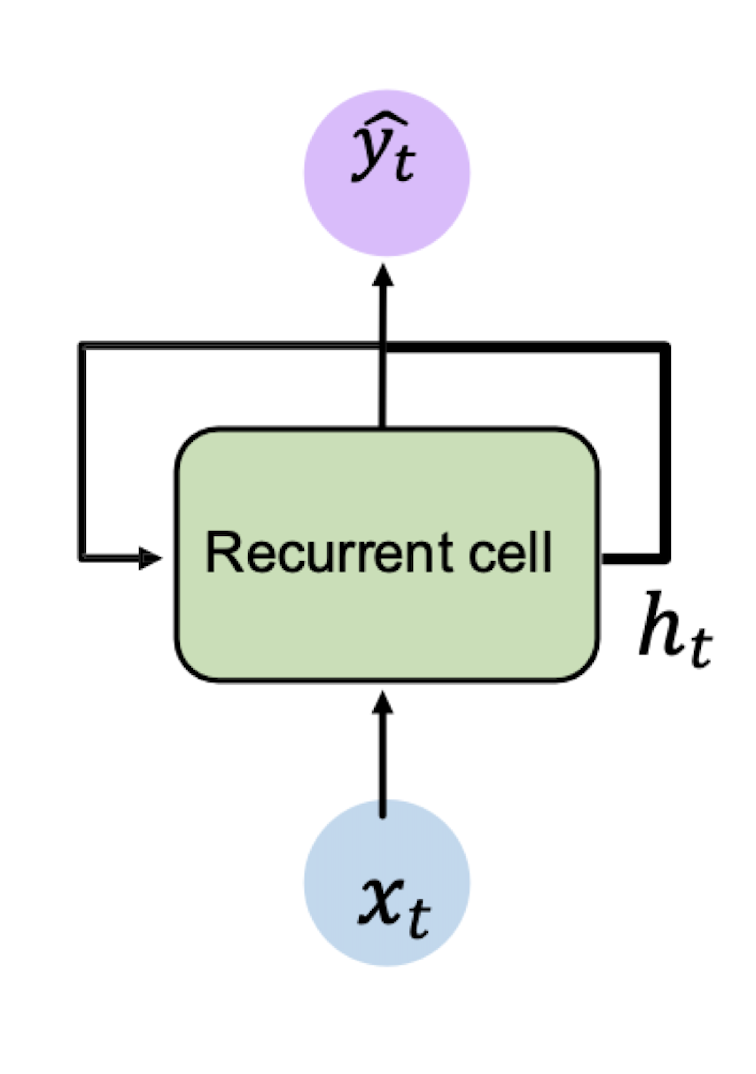
\includegraphics[width=0.32\textwidth]{figure/Recurrency_RNN.png}
    \caption{Rappresentazione della cella di ricorrenza, che integra input corrente e stato precedente attraverso la catena di retroazione.}
    \label{fig:recurrency_cell}
\end{figure}
Questo comportamento si può formalizzare tramite la seguente equazione:
\begin{equation}
    h_t = f_W(x_t, h_{t-1})
\end{equation}

Dove:
\begin{itemize}
    \item $h_t$ rappresenta lo stato nascosto corrente,
    \item $x_t$ è l'input al tempo $t$,
    \item $h_{t-1}$ è lo stato precedente,
    \item $f_W$ è una funzione non lineare parametrizzata dai pesi $W$.
\end{itemize}

Un esempio semplificato di utilizzo in pseudocodice Python è il seguente:
\vspace{0.5em}
\begin{python}
my_rnn = RNN()
hidden_state = [0, 0, 0, 0]

sentence = ["I", "love", "recurrent", "neural"]
for word in sentence:
    prediction, hidden_state = my_rnn(word, hidden_state)

nextWordPrediction = prediction
# >>> "networks!"
\end{python}
\vspace{0.5em}
Matematicamente, l'aggiornamento dello stato nascosto e il calcolo dell'output possono essere espressi così:
\begin{equation}
    h_t = \tanh(W_{hh}^T\,h_{t-1} + W_{xh}^T\,x_t) \qquad \hat{y}_t = W_{hy}^T\,h_t
\end{equation}

Come visibile nella Figura~\ref{fig:rolledRNN}, una RNN può essere vista come una rete "srotolata" nel tempo, dove ogni copia della cella condivide i medesimi parametri, ma riceve input e stato differenti. Questo riduce il carico computazionale rispetto a una rete profonda convenzionale e consente di modellare sequenze con efficienza. Inoltre, questa struttura consente di valutare la funzione di costo per ciascun intervallo temporale, rendendo esplicito come il modello gestisca la dipendenza tra istanti.

\subsection{Modellazione della sequenza}

La modellazione temporale può variare in base al tipo di task e al modo in cui si desidera produrre l'output. In Figura~\ref{fig:seqMod} sono illustrate diverse strategie:

\begin{itemize}
    \item \textbf{Many-to-One}: intera sequenza come input e un solo output finale (es. sentiment analysis);
    \item \textbf{One-to-Many}: un input iniziale e sequenza di output (es. image captioning);
    \item \textbf{Many-to-Many}: input e output sequenziali (es. machine translation).
\end{itemize}

\begin{figure}
    \centering
    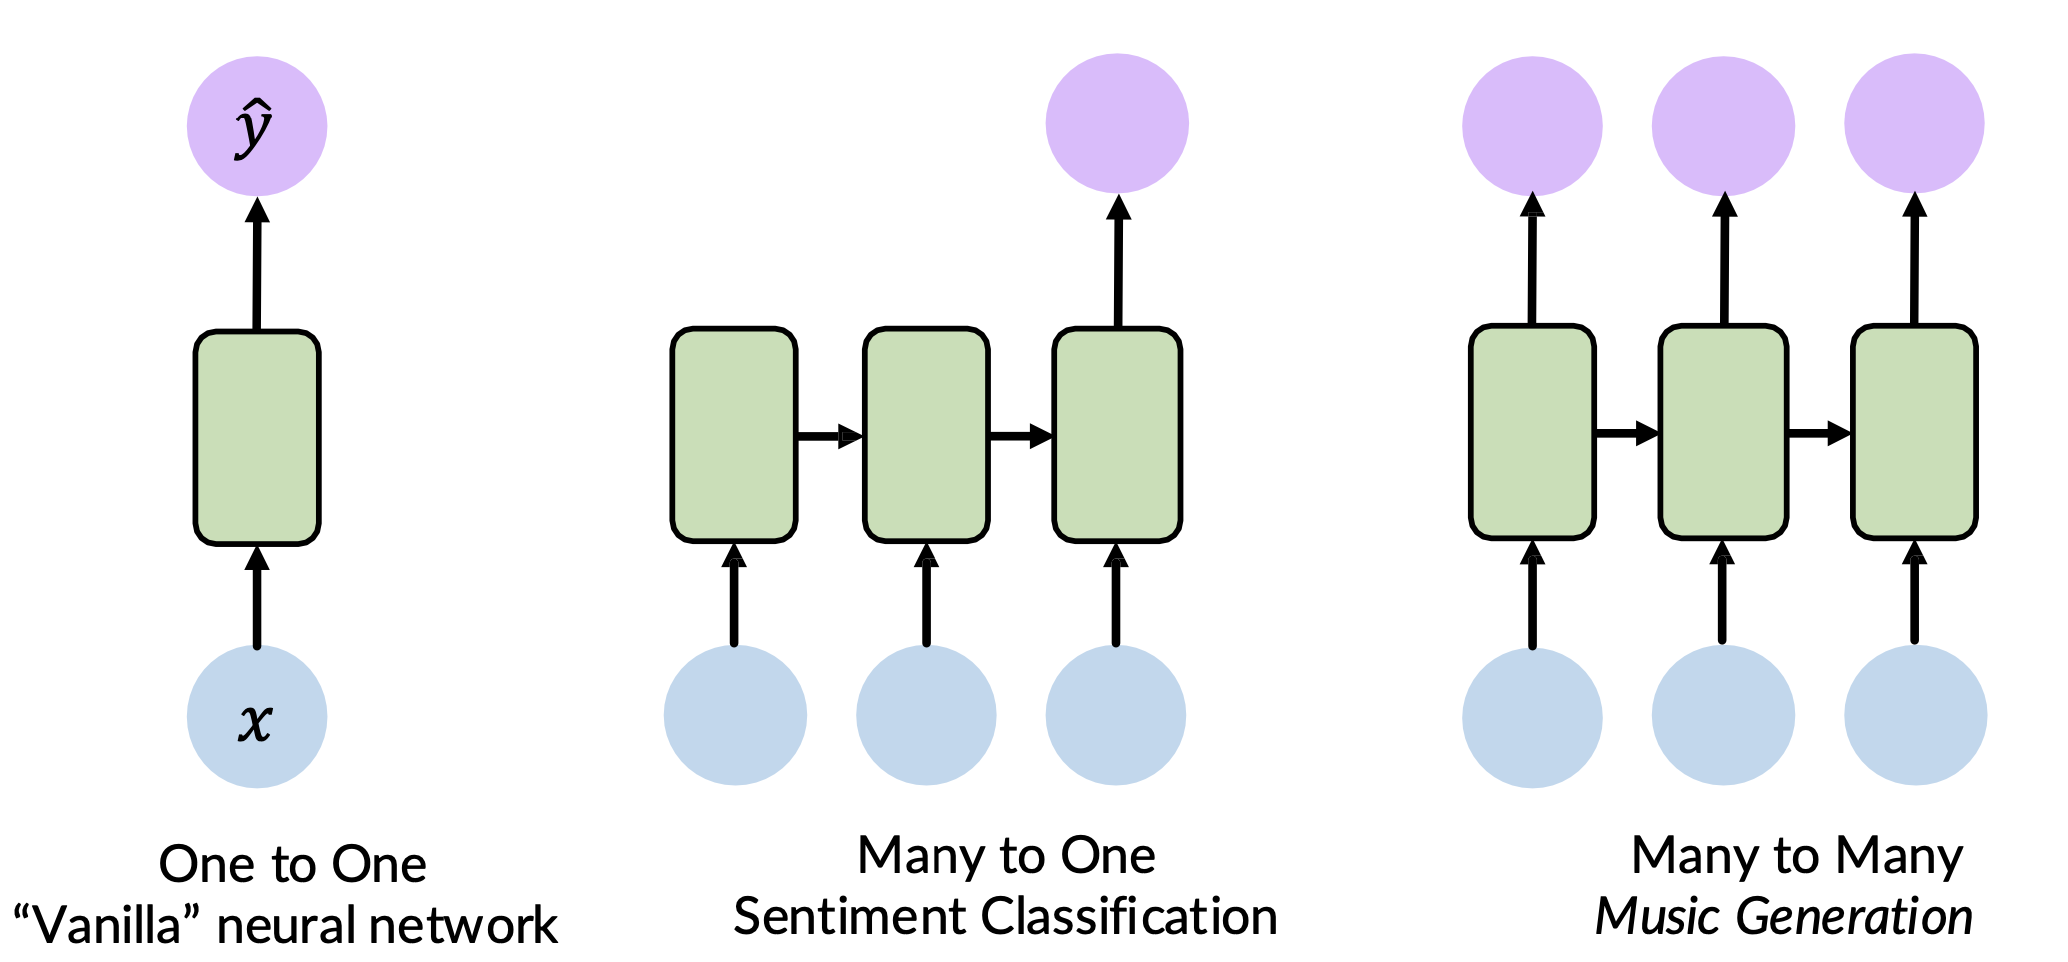
\includegraphics[width=0.85\textwidth]{figure/SequenceModeling.png}
    \caption{Esempi di modellazione della sequenza in RNN, adattabili al tipo di problema.}
    \label{fig:seqMod}
\end{figure}

\section{Backpropagation Through Time}

Quando si applica l'algoritmo di backpropagation a una RNN, lo si estende lungo la dimensione temporale: tale tecnica prende il nome di \textbf{Backpropagation Through Time} (BPTT). A ogni istante, la rete produce un output e aggiorna lo stato nascosto; durante la retropropagazione, vengono calcolati i gradienti a ritroso su tutti i \textit{timestep}, condividendo i pesi e sommando i contributi al gradiente.

\begin{equation}
    \frac{\partial L}{\partial W_{hh}} = \sum_{t = 1}^T \frac{\partial L_t}{\partial W_{hh}}
\end{equation}

Tuttavia, poiché lo stato nascosto $h_t$ dipende ricorsivamente da tutti gli stati precedenti, la derivata totale si espande in una lunga catena:
\begin{equation}
    \frac{\partial L}{\partial W} = \sum_{t=1}^T \frac{\partial L_t}{\partial h_t} \cdot \frac{\partial h_t}{\partial h_{t-1}} \cdots \frac{\partial h_1}{\partial W}
\end{equation}

\begin{figure}[!ht]
\centering
\begin{tikzpicture}[
  rnn/.style={draw, rectangle, rounded corners=5pt, minimum height=1.2cm, minimum width=1.8cm, fill=blue!10},
  arrowfwd/.style={->, thick, blue},
  arrowbwd/.style={->, thick, red, dashed},
  every node/.style={font=\small}
]

\node[rnn] (rnn0) at (0,0) {RNN$_0$};
\node[rnn, right=of rnn0] (rnn1) {RNN$_1$};
\node[rnn, right=of rnn1] (rnn2) {RNN$_2$};

\node[above=0.6cm of rnn0] (x0) {$x_0$};
\node[above=0.6cm of rnn1] (x1) {$x_1$};
\node[above=0.6cm of rnn2] (x2) {$x_2$};

\node[below=0.6cm of rnn0] (y0) {$\hat{y}_0$};
\node[below=0.6cm of rnn1] (y1) {$\hat{y}_1$};
\node[below=0.6cm of rnn2] (y2) {$\hat{y}_2$};

\draw[arrowfwd] (x0) -- (rnn0);
\draw[arrowfwd] (x1) -- (rnn1);
\draw[arrowfwd] (x2) -- (rnn2);

\draw[arrowfwd] (rnn0) -- (rnn1);
\draw[arrowfwd] (rnn1) -- (rnn2);

\draw[arrowfwd] (rnn0) -- (y0);
\draw[arrowfwd] (rnn1) -- (y1);
\draw[arrowfwd] (rnn2) -- (y2);

\draw[arrowbwd] (rnn2.south west) to[out=210,in=330] (rnn1.south east);
\draw[arrowbwd] (rnn1.south west) to[out=210,in=330] (rnn0.south east);

\end{tikzpicture}
\caption{Illustrazione della Backpropagation Through Time (BPTT), in cui gli errori si propagano all’indietro lungo la sequenza temporale.}
\end{figure}

Questa struttura porta inevitabilmente a due problemi noti:
\begin{itemize}
    \item \textbf{Vanishing Gradient:} i gradienti si riducono esponenzialmente man mano che si propaga l’errore, impedendo l’apprendimento delle dipendenze a lungo termine.
    \item \textbf{Exploding Gradient:} i gradienti crescono esponenzialmente, destabilizzando l’ottimizzazione.
\end{itemize}

In entrambi i casi, il modello fatica a gestire sequenze molto lunghe o con relazioni temporali distanti. Per risolvere queste problematiche, sono state introdotte le \textbf{Gated Cells}, che vedremo nella prossima sezione.

\section{Gated Cell}
L'idea alla base delle \textbf{Gated Cell} è quella di utilizzare unità ricorrenti più sofisticate, in grado di controllare dinamicamente quali informazioni devono essere mantenute o dimenticate lungo la sequenza temporale. Questo approccio risolve i limiti delle RNN standard nel memorizzare informazioni a lungo termine. Nel 1997, Hochreiter e Schmidhuber introdussero le \textit{Long Short Term Memory} (LSTM), che grazie a strutture semplici ma potenti — come moduli lineari e logistici con operazioni moltiplicative — riuscivano a decidere quando scrivere, leggere o conservare un'informazione in memoria, a seconda dello stato di specifici \textit{gate}. Diverse architetture implementano queste logiche con variazioni e nomi differenti. In questo capitolo ci concentreremo su due tra le più diffuse: le \textbf{Long Short Term Memory} (LSTM) e le \textbf{Gated Recurrent Unit} (GRU).

\begin{figure}[!ht]
    \centering
    \begin{tikzpicture}[scale=0.8]
    \node[draw=black, fill=darkpastelgreen!60, text=white, rounded corners=15pt, thick, minimum width=6cm, minimum height=3cm, align=center, font=\bfseries\large] 
    at (0,0) {Gated cell\\LSTM, GRU, etc...};
    \end{tikzpicture}
\end{figure}

\subsection{Long Short Term Memory Networks}
In una RNN classica, i blocchi ripetuti sono costituiti da semplici nodi computazionali. Le LSTM, invece, introducono una struttura interna più articolata (Figura~\ref{fig:LSTMSchema}), capace di gestire efficacemente il flusso informativo nel tempo. Questa architettura permette alla rete di conservare informazioni anche per sequenze molto lunghe. In \texttt{TensorFlow}, una cella LSTM può essere facilmente implementata con il comando \texttt{tf.keras.layers.LSTM(numUnits)}. Il cuore delle LSTM sono i \textit{gate}, che regolano l'informazione tramite funzioni sigmoidi e moltiplicazioni punto a punto:

\begin{figure}
    \centering
    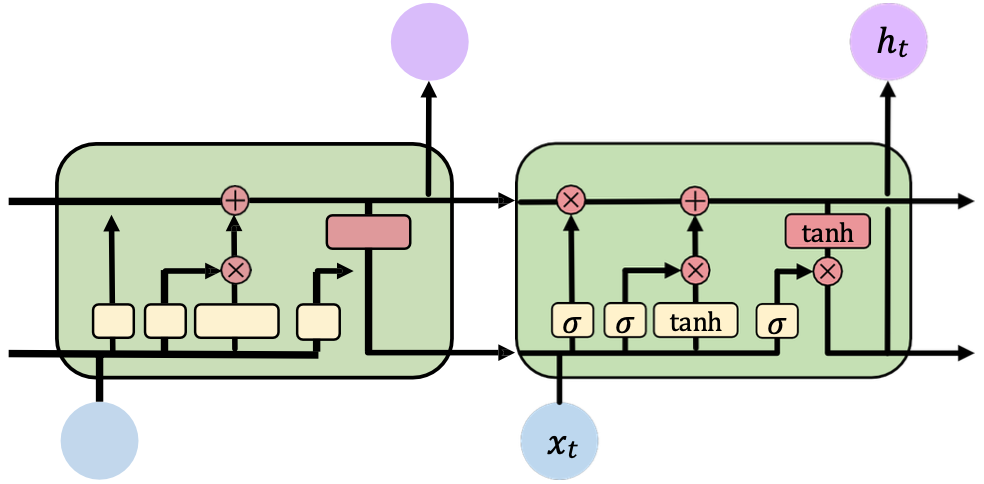
\includegraphics[width=0.85\textwidth]{figure/LSTMSchema.png}
    \caption{Rappresentazione della cella LSTM, che interagisce con un timestep precedente}
    \label{fig:LSTMSchema}
\end{figure}

\subsubsection{Forget Gate}
Il \textit{forget gate} decide quali informazioni dello stato precedente devono essere mantenute. Per farlo, combina l'input corrente con lo stato nascosto precedente, e li elabora tramite una funzione sigmoide. I valori prodotti, compresi tra 0 e 1, indicano il grado con cui ciascun elemento della memoria deve essere conservato: più vicino a 0 indica dimenticare, più vicino a 1 conservare.

\begin{figure}[!ht]
    \centering
    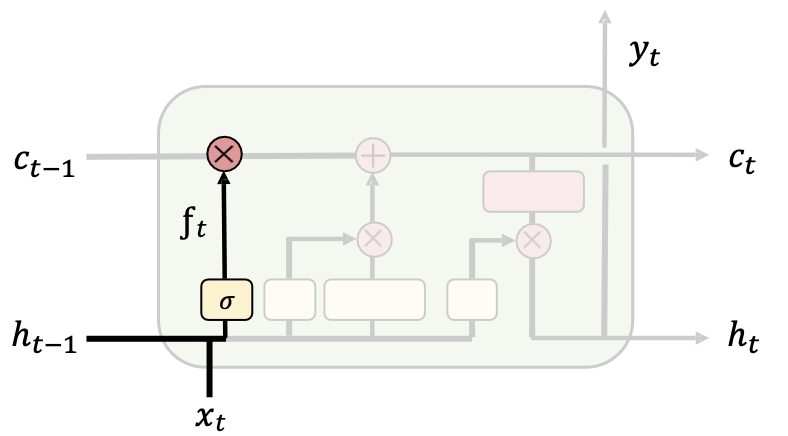
\includegraphics[width=0.55\textwidth]{figure/ForgetLSTM.png}
    \caption{Rappresentazione del gate Forget della cella LSTM}
    \label{fig:LSTMForget}
\end{figure}

\subsubsection{Store (o Input Gate)}
Lo \textit{store gate}, o \textit{input gate}, determina quali nuove informazioni devono essere aggiunte alla memoria della cella. Anche qui, input e stato nascosto precedente sono elaborati da due percorsi:
\begin{itemize}
    \item Una funzione sigmoide, che seleziona le componenti informative da aggiornare;
    \item Una funzione $\tanh$, che normalizza i nuovi valori da memorizzare in un intervallo tra -1 e 1.
\end{itemize}
Il prodotto tra questi due risultati indica quali parti della nuova informazione saranno effettivamente aggiunte allo stato interno.

\begin{figure}[!ht]
    \centering
    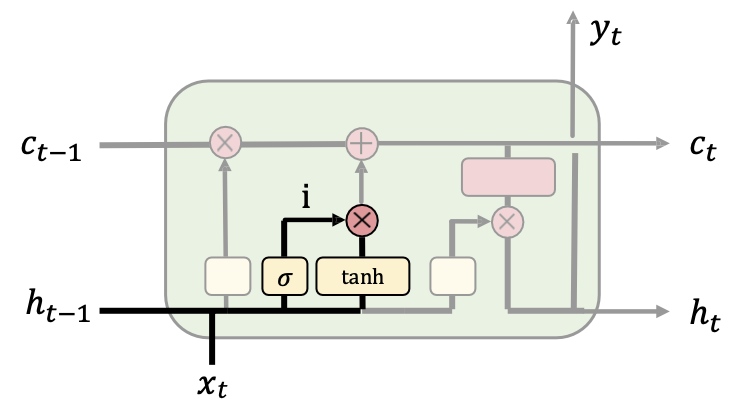
\includegraphics[width=0.55\textwidth]{figure/StoreLSTM.png}
    \caption{Rappresentazione del gate Store della cella LSTM}
    \label{fig:LSTMStore}
\end{figure}

\subsubsection{Update Gate}
L’\textit{update} rappresenta il cuore del funzionamento della LSTM. Qui lo stato della cella viene aggiornato combinando:
\begin{itemize}
    \item Lo stato precedente, pesato dal forget gate;
    \item Le nuove informazioni, selezionate dallo store gate.
\end{itemize}
La somma dei due produce il nuovo stato della cella, considerando tutti i valori che adesso la rete neurale ritiene rilevanti.

\begin{figure}[!ht]
    \centering
    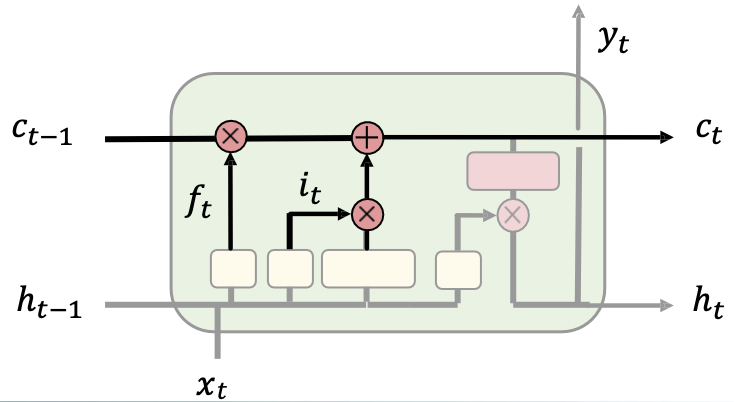
\includegraphics[width=0.55\textwidth]{figure/UpdateLSTM.png}
    \caption{Rappresentazione del gate Update della cella LSTM}
    \label{fig:LSTMUpdate}
\end{figure}

\subsubsection{Output Gate}
Infine, l’\textit{output gate} decide quale informazione deve essere trasmessa al prossimo timestep, ovvero il nuovo stato nascosto. L'input e lo stato nascosto precedente vengono processati da una funzione sigmoide, mentre lo stato interno aggiornato attraversa una funzione $\tanh$. Il prodotto punto a punto di questi due risultati rappresenta l'output finale della cella.

\begin{figure}[!ht]
    \centering
    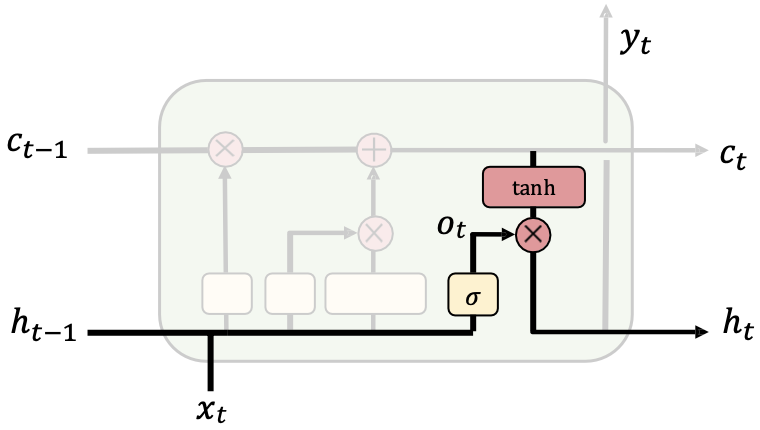
\includegraphics[width=0.55\textwidth]{figure/OutputLSTM.png}
    \caption{Rappresentazione del gate Output della cella LSTM}
    \label{fig:LSTMOutput}
\end{figure}

\subsubsection{Backpropagation solved}
Grazie alla struttura interna della cella, le LSTM mitigano i problemi del gradiente che scompare o esplode: le informazioni vengono propagate tramite somme e moltiplicazioni punto a punto, evitando lunghe catene di moltiplicazioni tra matrici che potrebbero alterare drasticamente i gradienti.

\subsection{Gated Recurrent Unit}
Le \textbf{Gated Recurrent Unit} (GRU) sono una versione semplificata delle LSTM, ma mantengono ottime capacità di apprendimento del contesto. Le GRU impiegano due gate:
\begin{itemize}
    \item Il \textbf{reset gate}, che decide quanto dello stato precedente deve essere dimenticato;
    \item L’\textbf{update gate}, che controlla quanto del nuovo contenuto deve essere incorporato nel nuovo stato nascosto.
\end{itemize}

\begin{figure}[hbtp]
    \centering
    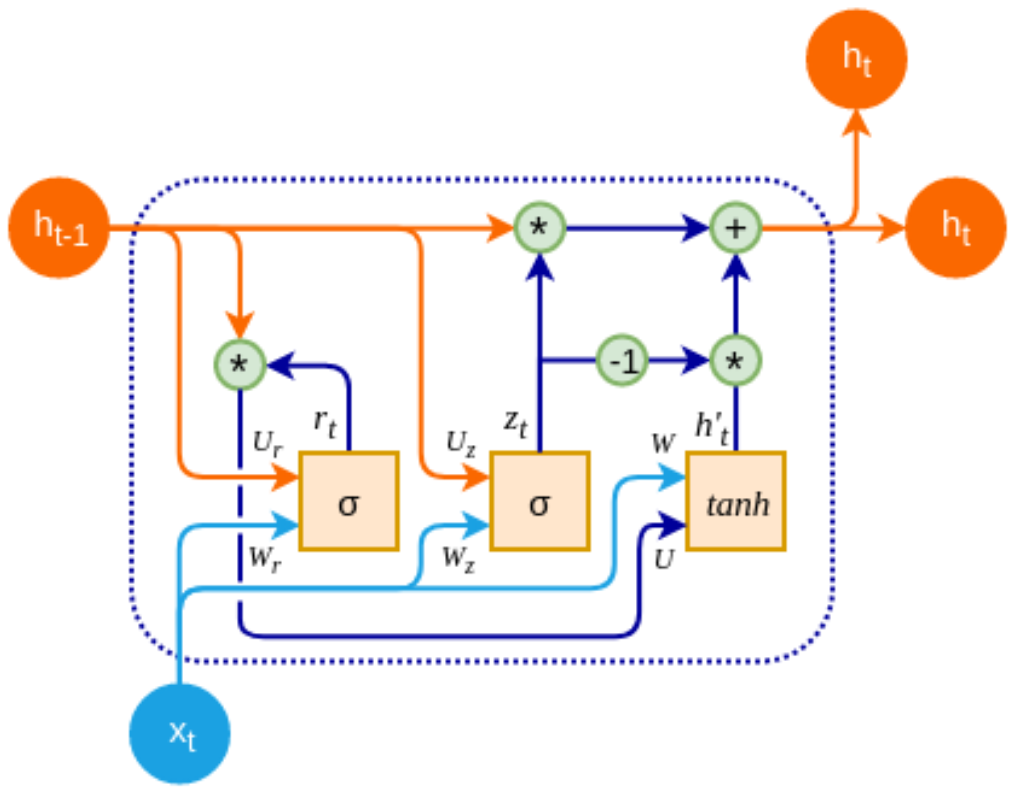
\includegraphics[width=0.70\textwidth]{figure/GNU.png}
    \caption{Rappresentazione della cella GNU, con tutti i suoi gate}
    \label{fig:GNU}
\end{figure}

\subsection{Applicazioni}
Le RNN — e in particolare le loro varianti LSTM e GRU — trovano impiego in moltissimi ambiti: generazione musicale, analisi del sentimento, traduzione automatica, e altro ancora. Queste applicazioni si basano spesso sul \textbf{meccanismo dell'attenzione}. Il \textit{meccanismo dell’attenzione} consente alla rete di concentrarsi sulle parti più rilevanti della sequenza, simulando l'apprendimento umano del linguaggio. Proprio come un bambino associa significati alle parole tramite contesto e ripetizione, l’attenzione permette alla rete di catturare relazioni semantiche tra parole, senza alcuna codifica esplicita delle regole grammaticali.\marginpar{\href{https://arxiv.org/pdf/1706.03762}{"Attention Is All You Need", by Ashish Vaswani et al. (2017)~\cite{vaswani2017attention}}}A ogni parola è associato un vettore numerico molto lungo. Questi vettori possono essere visualizzati come punti in uno spazio semantico, la cosa straordinaria è che la vicinanza tra punti, riflette affinità semantiche tra parole.
\begin{figure}
    \centering
    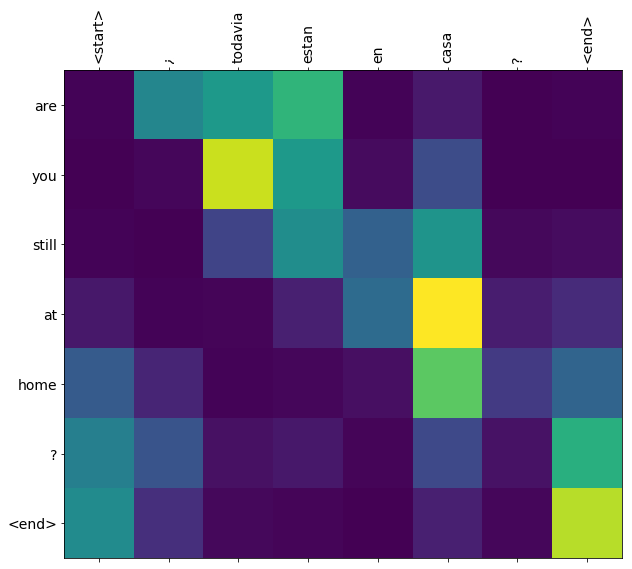
\includegraphics[width=0.50\textwidth]{figure/AttentionEx.png}
    \caption{Rappresentazione del meccanismo dell'attenzione in un compito di traduzione: le zone più gialle indicano alta probabilità di corrispondenza tra parole.}
    \label{fig:AttEx}
\end{figure}
L'algoritmo dell'attenzione calcola il prodotto scalare tra ogni parola e tutte le altre, identificando le relazioni più rilevanti. Questo approccio non è limitato al linguaggio: può essere applicato anche a note musicali, pixel o altri dati sequenziali.

\subsection{Bi-LSTM}
Le \textbf{Bi-LSTM} (Bidirectional LSTM) estendono le LSTM standard eseguendo due elaborazioni:
\begin{enumerate}
    \item Una in avanti, dalla prima all'ultima parola;
    \item Una all’indietro, dall’ultima alla prima parola.
\end{enumerate}
I risultati vengono poi combinati (di solito tramite concatenazione o somma), fornendo un contesto bidirezionale. Questo è particolarmente utile, ad esempio, per prevedere una parola mancante in una frase: serve sia il contesto passato che futuro.
\begin{figure}
    \centering
    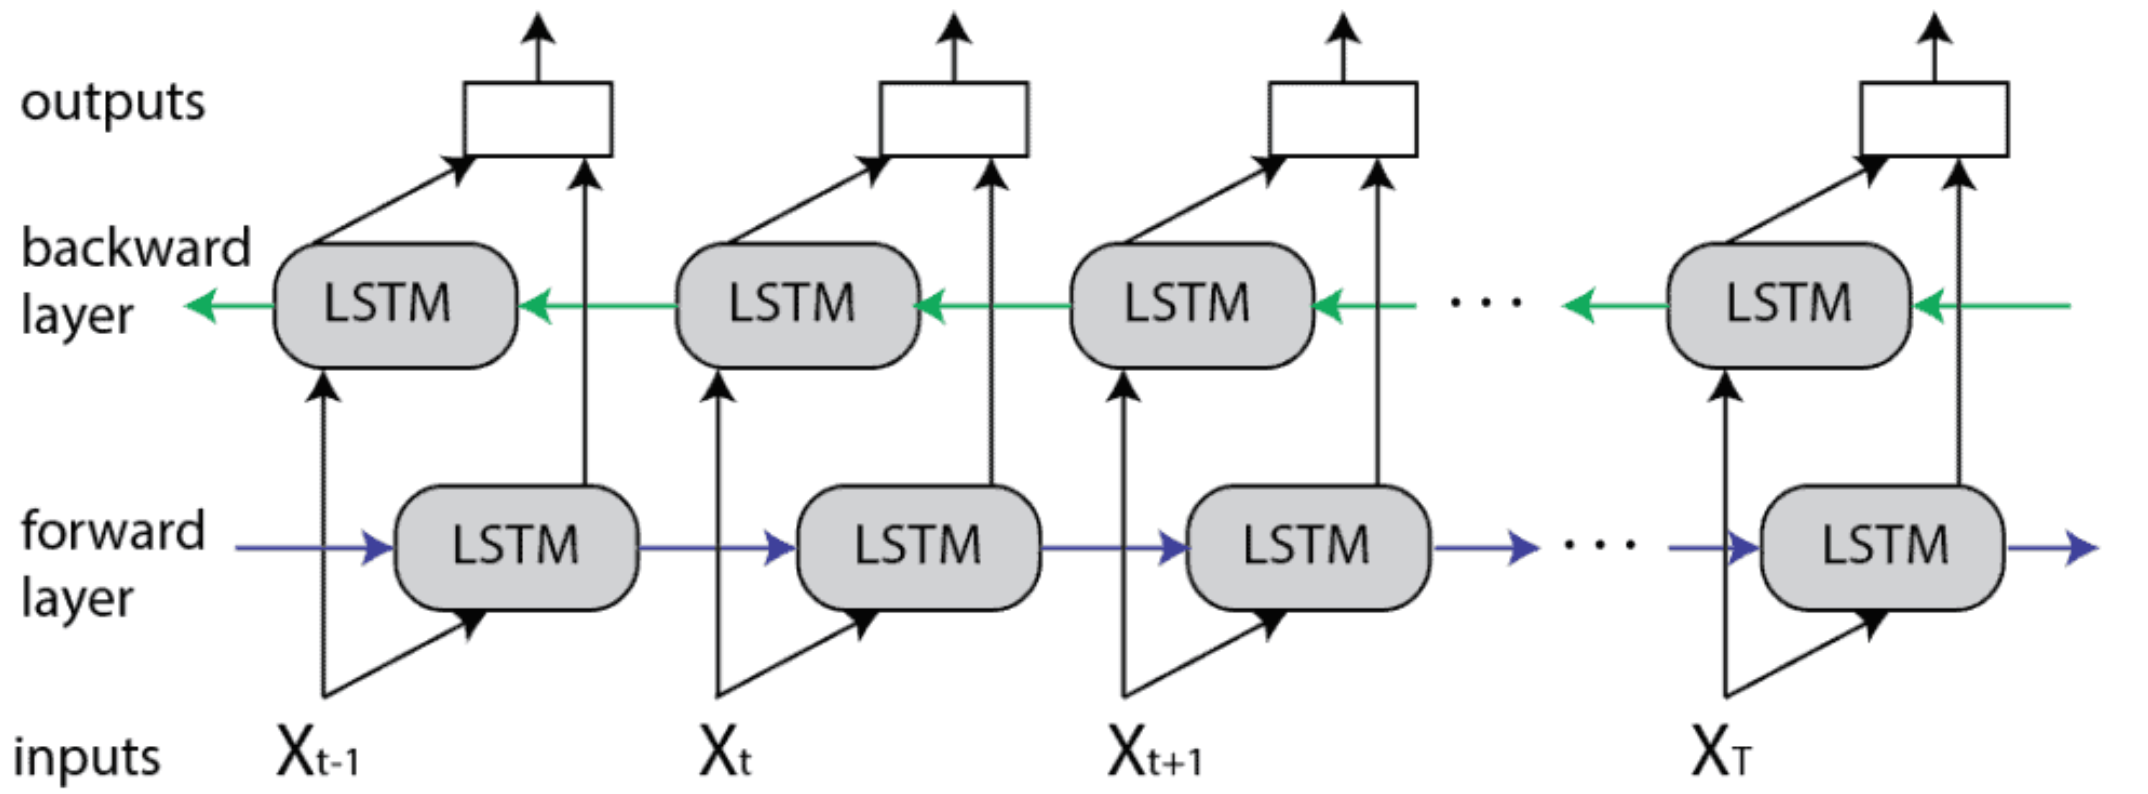
\includegraphics[width=0.8\textwidth]{figure/Bi-LSTM.png}
    \caption{Architettura di una Bi-LSTM}
    \label{fig:bilstm}
\end{figure}
Questa potenza ha un costo: due reti LSTM devono essere addestrate simultaneamente, il che comporta un maggiore uso di memoria e tempi di addestramento più lunghi.

\subsection{Bi-LSTM con Attenzione}
Un limite delle Bi-LSTM è che, nonostante processino la sequenza in entrambe le direzioni, alla fine restituiscono un singolo vettore che riassume l'intera sequenza. Questo può essere problematico se la sequenza è molto lunga o se alcune parti sono più rilevanti di altre. Il \textbf{meccanismo dell'attenzione} risolve questo problema: assegna un peso $\alpha_t$ a ciascun passo temporale, indicando quanto ogni stato nascosto deve contribuire all'output finale.

\begin{figure}[hbtp]
    \centering
    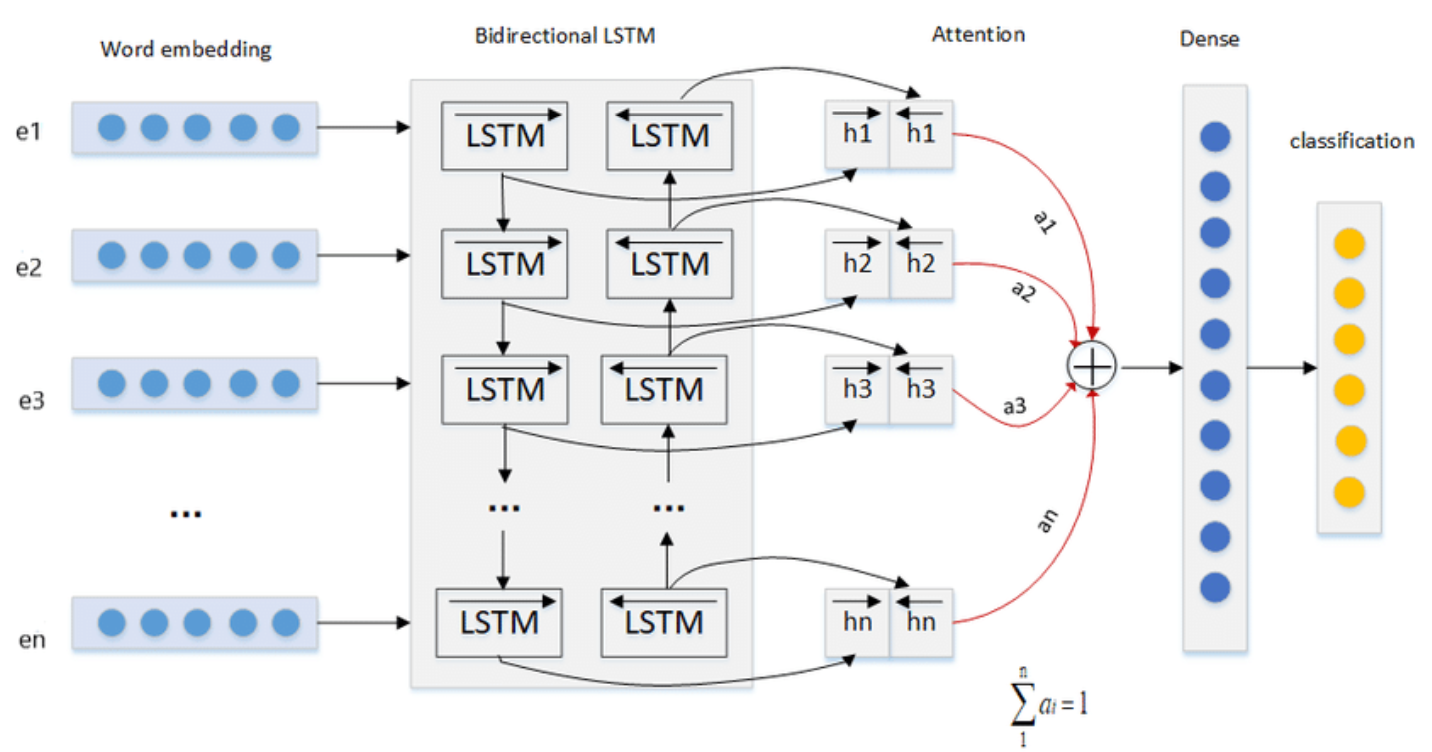
\includegraphics[width=0.8\textwidth]{figure/Bi-LSTMAtt.png}
    \caption{Architettura di una Bi-LSTM con meccanismo di attenzione}
    \label{fig:bilstmatt}
\end{figure}